\section{Synchronization (PPT+PPS)}
Fast mode \approx $50\mu s$. Accurate mode prohibits $20hz$ refresh rate.
Verified using oscilloscope and analog output.
Cameras report ptp offset, but without a proper oscilloscope it is hard to verify if this is correct.

\subsection{Reduce trigger latency}
It is possible to reduce the trigger latency of the cameras, which results in a lower synchronization offset.
This can be acheived by setting the \code{TriggerLatency} node to \code{OneLine}.
This reduces the average trigger offset down to $10\mu s$.
Unfortunately, this option becomes unavailable while the \code{TriggerOverlap} node is set to \code{set_PreviousFrame}, which is requiered for the cameras to


\subsection{Validation}
\begin{table}[H]
    \centering
    \begin{tabular}{c}
        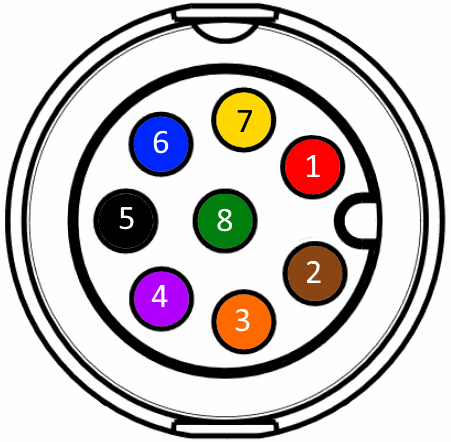
\includegraphics[width=0.3\textwidth]{figures/m8-pin-layout.png}
        \\
        \small
        \begin{tabular}{ |l|l| }
            \hline
            \textbf{Pin} & \textbf{Pin Description}                          \\
            \hline
            1 (Red)      & $V_{AUX}$ (12-24V DC Power Input)                 \\
            2 (Brown)    & Non-isolated bi-directional GPIO channel (Line 2) \\
            3 (Orange)   & VDD GPIO (2.5V Power Output) (Line 4)             \\
            4 (Purple)   & Non-isolated bi-directional GPIO channel (Line 3) \\
            5 (Black)    & GND (Camera GND)                                  \\
            6 (Blue)     & OPTO GND (Opto-isolated Reference)                \\
            7 (Yellow)   & OPTO OUT (Opto-isolated Output) (Line 1)          \\
            8 (Green)    & OPTO IN (Opto-isolated Input) (Line 0)            \\
            \hline
        \end{tabular}
    \end{tabular}
    \caption{\cam \gls{gpio} connector \cite{lucidvisionlabsTritonMPPolarized2020}}

\end{table}


\begin{figure}[H]
    \centering
    \subcaptionbox{Synchronization at $25ms$ resolution}{
        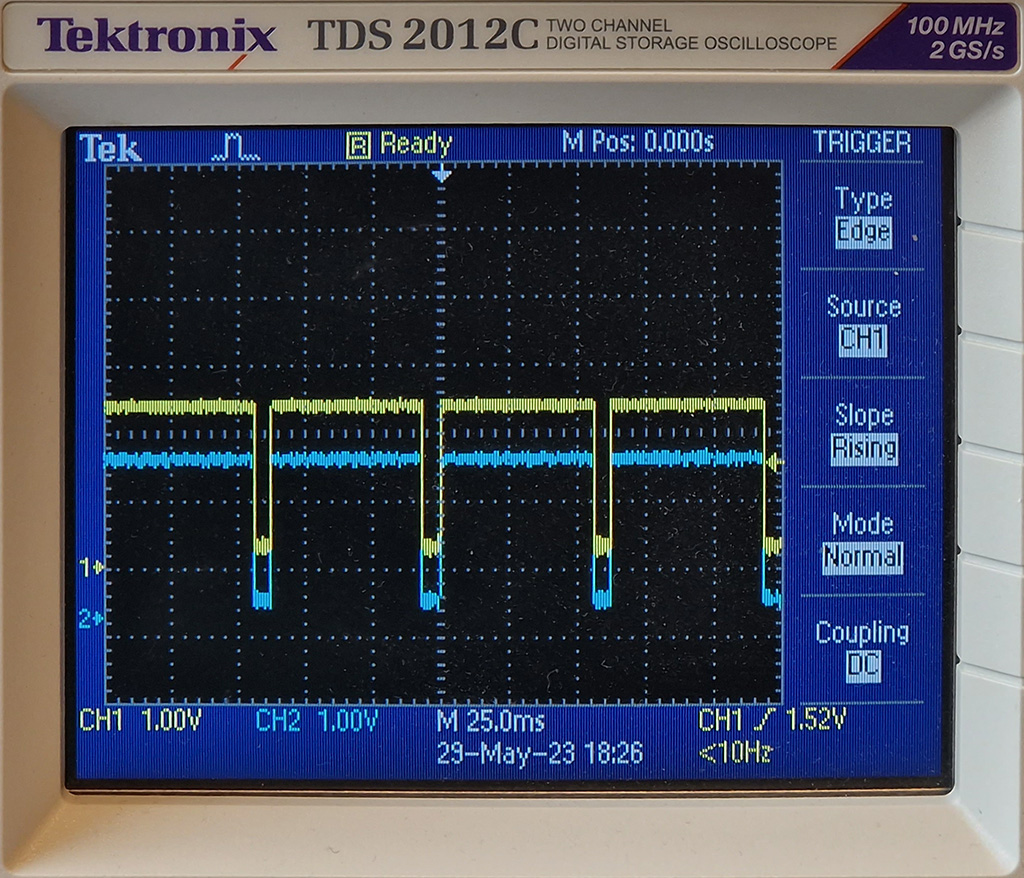
\includegraphics[width=0.8\textwidth]{figures/synchronization/ms.jpg}
    }
    \subcaptionbox{Synchronization at $10\mu s$ resolution}{
        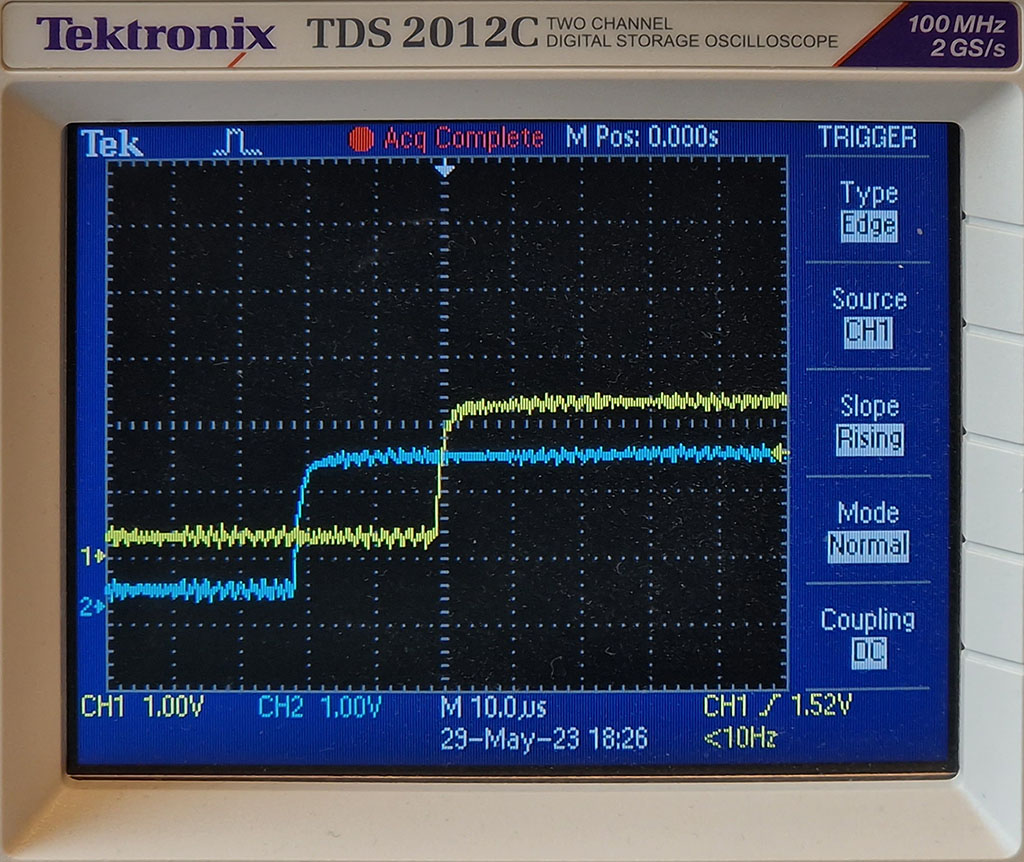
\includegraphics[width=0.8\textwidth]{figures/synchronization/us.jpg}
    }
    \caption{Measured synchronization offset of $22\mu s$ between the two cameras.}
\end{figure}

